\documentclass[hidelinks]{article}
\usepackage{tikz}
\usepackage{physics}
\usepackage{bbm}
\usepackage{pstricks}
\usepackage{bm}
\usepackage{amsmath}
\usepackage{graphicx}
\usepackage{mathtools}
\usepackage{amsfonts}
\usepackage{hyperref}
\usepackage{bbm}
\usepackage{seqsplit}

%opening
\title{Frog on a Garden Path}
% See https://arxiv.org/pdf/1108.0337.pdf
\author{Harry Mallinson}

\begin{document}

\maketitle


\begin{abstract}
I used this problem in one of an ongoing series of  data science internal training sessions, summer 2021. It highlights nicely how large performance benefits can come from simply rolling up one's mathematical sleeves a little.
\end{abstract}

\section{Problem Statement}
\subsection{Frog 1}

\textbf{Difficulty:} 2/5 \\

A frog sits at the start of a garden path of length 10m.  Each hop it can jump either 1, 2 or 3 metres exactly.  How many different ways can it reach the end of the garden path without overshooting?  
\\

\textit{Note}: The frog must end exactly at the end of the path. For example, a hop sequence of 3,3,3,3 is  invalid, as the frog ends up hopping 12m, not 10m.

\textit{Note}: Hopping e.g. 3, 3, 3, 1 is counted as different to hopping 3, 3, 1, 3 and so on.

\textit{Note}: The frog starts at the 0m mark.

\subsection{Frog 2}

\textbf{Difficulty:} 3/5\\

Solve the general case of \textbf{Frog 1}, where the length of the garden path is $N$, and the frog can jump $1, 2, 3, \dots, k$ metres per jump (i.e. the frog can jump any integer distance between 1 and $k$ metres).

If you have coded your solution, check its efficiency by making sure it can calculate $N=100, k=25$ in under a second. The correct result is 633824582314588604117041545216. \\


Push the boat out: see if you can calculate $N=900, k=300$ in under a second. The correct result is: \\

\seqsplit{4226356249085321970818718279332132852150778608288972177023685672213391220453798875795337423636543278788203143456775509834095840855975089871860087480189730594682178682543044117377244106228260440730347272120364229185899239035975403380259737710579931032227208688810246275072}.



\newpage


\section{Solution}

I'll present three ways you might approach this. 

First note that the question is equivalent to asking you to enumerate the possible \textbf{compositions} of integer $N$ with largest part of size $k$ - in the non-general case above we have $N=10$ and $k=3$.  To understand compositions we must first understand \textbf{partitions}.

A \textbf{partition} of an integer is a way of writing that integer as a sum of positive integers. Two partitions of an integer are considered identical if they differ only in the order of their parts (their summands). For example, one partition of 6 could be $3+2+1$ which is identical to the partition $2+3+1$.

A \textbf{composition} of an integer is simply an ordered partition of that integer - that is, a composition is identical to a partition except that the order of the parts matters. For example, $3+2+1$ and $2+3+1$ are distinct compositions of 6. 

\textbf{Frog 1} is equivalent to asking for the total possible compositions of 10 with no part greater than 3, and \textbf{Frog 2} is equivalent to asking for the total possible compositions of any integer $N$ with no part greater than integer $k$.


\subsection{Fibonacci}

We wish to find the number of compositions of some integer $N$ with possible parts $\{1,\dots,k\}$. Write this as $C_N^k$.

If $k=1$ the only possible composition of N is $1+1+\dots+1$, which is just the composition of $C_{N-1}^1$ (so $N-1$ $1$s) with a $1$ appended.  If $k=2$ we can do similarly: we can append a 1 to the compositions of $C_{N-1}^2$ and a 2 to the compositions of $C_{N-2}^2$. From this observation we have our solution.  Consider the compositions of increasing $N$ for $k=2$, where for ease I've written some general composition $a+b+c+d$ as $(a,b,c,d)$:

\begin{center}
	\begin{tabular}{| r | l |}
		\hline
		Element & Compositions \\ [0.5ex]
		\hline
		$C_0^2$ & ()\\
		$C_1^2$ & (1) \\
		$C_2^2$ & (1,1), (2)\\
		$C_3^2$ & (1,1,1), (2,1), (1,2) \\ 
		$C_4^2$ & (1,1,1,1), (2,1,1), (1,2,1), (1,1,2), (2,2) \\
		\hline
	\end{tabular}
\end{center}

Notice that the compositions of $C_1^2$ are just all the compositions of $C_0^2$ with a $1$ appended. Notice then that the compositions of $C_2^2$ are just all the compositions of $C_1^2$ with a $1$ appended, and then all the compositions of $C_0^2$ with a $2$ appended.  Finally, the compositions of $C_3^2$ are just all the compositions of $C_2^2$ with a $1$ appended, and all those of $C_1^2$ with a $2$ appended. We can't go back and append a $3$ to the compositions of $C_0^2$ as the max part size is in the above table is $k=2$.

For general $C_N^k$ we can then just append 1s to the $C_{N-1}^k$ compositions, 2s to the $C_{N-2}^k$ compositions and so on to appending $k$s to the $C_{N-k}^k$ compositions.  As appending does not change the total number of compositions for each $C_{N-i}^k$, we can just write $C_N^k$ (the number of compositions of $N$ with max part size $k$) as 

\begin{equation}
C_N^k = C_{N-1}^k + C_{N-2}^k + \dots + C_{N-k}^k
\end{equation}
and as we know the boundary condition $C^k_0=1$  (there is only one composition of 0, the empty sequence) and $C^k_{N<0}=0$ (there are no compositions of the negatives) this just defines a (certain generalisation of) the Fibonacci sequence. 

We have then that the number of compositions of integer $N$ of max part size $k$ is given by the general Fibonacci number
\begin{equation}
F_n^k = 
\begin{cases}
0 & \text{if }n<0; \\
1 & \text{if }n=0; \\
\sum_{i=1}^kF^k_{n-i} & \text{if }n>0.
\end{cases}
\end{equation}

This suffices to solve \textbf{Frog 2}. To solve \textbf{Frog 1} we just want $F_{10}^3=274$.

Continuing along this path you can get all sorts of interesting results - the number of times some part of size $j$ appears, or the total number of parts present in the set of compositions, or (relatedly) the average number of parts per composition.  


~\\[8pt]
\subsection{Adjacency Matrices}

We can represent the frog scenario as an ordered graph, with node 0 (the starting point) connected to nodes 1, 2 and 3 representing the possible jumps of 1, 2 and 3 metres (up to $k$ metres in the generalised question).  Node 1 connects to nodes 2, 3 and 4 and so on up to $k$. 

We can represent connected graphs in matrix form.  Consider the directed graph $G_1$ in \ref{G_1}.

\begin{figure}[h]
	\centering
	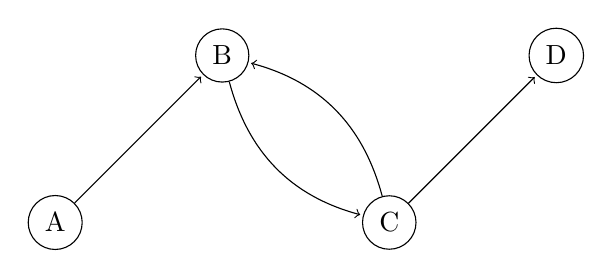
\begin{tikzpicture}[->,shorten >=1pt,auto,node distance=3cm,main node/.style={circle,draw}]
	
	\node[main node] (A) {A};
	\node[main node] (B) [above right of=A] {B};
	\node[main node] (C) [below right of=B] {C};
	\node[main node] (D) [above right of=C] {D};
	
	\path[every node/.style={font=\sffamily\small}]
	(A) edge node [left] {} (B)
	
	(C) edge node [right] {} (D)
	edge [bend right] node[right] {} (B)
	(B) edge [bend right] node [left] {} (C)
	;
	\end{tikzpicture}
	\caption{\textit{Directed Graph $G_1$}} \label{G_1}
\end{figure}
We can represent this as an \textbf{adjacency matrix }
\begin{equation}
\textbf{M} = 
\begin{pmatrix}
0  & 1 & 0 & 0 \\
0  & 0 & 1 & 0 \\
0  & 1 & 0 & 1 \\
0  & 0 & 0 & 0
\end{pmatrix}
\end{equation}
where $\textbf{M}_{ij}$ represents the number of connections from $i$ to $j$, for $A=0, B=1, \dots$.  If one starts at $A$ and stores one's position in a $1\cross4$ vector $\textbf{P}$, and takes all available paths at any time, then $\textbf{P}$ acting on $\textbf{M}$ $n$ times will determine your (possibly multiple) potential position(s) after $l$ moves.  For example
\begin{equation}
\begin{split}
\begin{pmatrix}
1 & 0 & 0 & 0
\end{pmatrix}
\textbf{M} & = \textbf{PM} \\
& =
\begin{pmatrix}
0 & 1 & 0 & 0
\end{pmatrix}
\end{split}
\end{equation}
which just codifies your position(s) after 1 move from $A$ (so here just ending up at $B$), and
\begin{equation}
(\textbf{PM})\textbf{M}=\textbf{PM}^2=
\begin{pmatrix}
0 & 0 & 1 & 0
\end{pmatrix}
\end{equation}
which just codifies your position(s) after 2 moves from $A$ (so here just ending up at $C$), and
\begin{equation}
\textbf{P}\textbf{M}^3=
\begin{pmatrix}
0 & 1 & 0 & 1
\end{pmatrix}
\end{equation}
which just codifies your position(s) after 3 move from $A$ (so here ending up at both $C$ and $D$).

Continuing this reasoning, we can see that $(\textbf{PM}^n)_i$ tells you the number of possible paths that end up at node $i$ after $n$ moves from node $A$ (as we started at node $A$).  Then we see that we can do away with $P$ altogether, as $(\textbf{M}^n)_{ij}$ represents the number of possible paths of length $n$ from node $i$ to node $j$.\footnote{For any starting position $M_{ij}$ - which, referring back to \textbf{P}, just has non-0 $j$ telling us the starting node - when multiplying its row $i$ by $M$, you can see that $M_{ij}$ will be ``caught''  by exactly those elements of $M$ in row $j$ that represent the connections from node $j$ onwards to some other (or same) node $l$.}  If you don't see this just play around with $\textbf{P}$ and $\textbf{M}$, referring back to the graph.

So, we have that an adjacency matrix \textbf{M} is a way of representing a graph $G$, with $M_{ij}$ telling you the number of direct connections from node $i$ to node $j$ of $G$, and that $(M^n)_{ij}$ gives the number of $n$-step connection from node $i$ to node $j$.  

In order to ``catch'' the frogs once they reach the final step of node 10 we connect node 10 to itself (otherwise every time a frog arrives at node 10 it would disappear on the next step, in our notation).  The adjacency matrix is then an $11\cross11$ matrix 


\begin{equation}
\text{\textbf{M}} = 
\begin{pmatrix}
0 & 1 & 1 & 1 & 0 & 0 & \dots &\\
0 & 0 & 1 & 1 & 1 & 0 & \dots &\\
0 & 0 & 0 & 1 & 1 & 1 & \dots &\\
&  &  &  & \ddots & \ddots & \ddots & \\
&   &   &   & \dots  & 0  & 0  &  1
\end{pmatrix}.
\end{equation}

$(M^{10})_{1,10}=274$ then gives us our answer as the total number of possible paths from node 0 to node 10. This suffices to solve \textbf{Frog 1}. Generalising this to finding the number of compositions of some integer $N$ with largest size $k$ is straightforward - we simply want $(M^N)_{1,N}$ for an appropriately constructed $\textbf{M}$.\footnote{Instead of each row containing a max of 3 $1$s, the rows will have a max of $k$ 1s.} This suffices to solve \textbf{Frog 2}.

\subsection{Generating functions}
For our purposes, it suffices to note that if we use the following ``generating'' function
\begin{equation}
f(x)=x^1+x^2+\dots+x^k
\end{equation}
then the total coefficient of $f(x)^r[x^N]$ (all terms of order $[x^N]$ in $f(x)^r$) will equal the number of compositions of $N$ with $r$ parts and max part size $k$.\footnote{Play a little with this if it's not clear - it all rests on the fact that $x^ax^b = x^{a+b}=x^bx^a$. Squaring $g(x)=x^1+x^2$ gives $g(x)^2 = x^{1+1}+x^{1+2}+x^{2+1}+x^{2+2} = x^2+2x^3+x^4$. This tells us that there is 1 composition of 2 with two parts, max part size 2 (just the $1+1$) as the coefficient of the $x^2$ term is 1. Similarly there are two compositions of 3 with two parts, max part size 2 (compositions $2+1$ and $1+2$) as the coefficient of the $x^3$ term is 2, and only 1 for 4 (composition $2+2$).}

That is, for $f(x)^r=(x^1+\dots+x^k)^r$, if we take only the $x^N$ terms from the expanded product, the coefficient will equal the number of compositions of $N$ of $r$ parts, with max part size $k$.\footnote{Another way to see this is to note that the expanded product will have every possible length $r$ product permutation (with repetition) of the $x^1, \dots, x^k$, which means that the powers of $x$ in the expanded product will be equal to every possible length $r$ \textit{summation} of just those powers $1, \dots, k$. Hence the coefficient in front of each $x^n$ must represent all the different ways to make up $n$ from exactly $r$ permutations (with repetition) of $1, \dots, k$.}

It is easy to show that
\begin{equation}
(1-x)\sum_{n=0}^kx^n=(1-x)(x^0+x^1+\dots+x^{k})=(1-x^{k+1})
\end{equation}
hence
\begin{equation}
\sum_{n=0}^kx^n=\frac{1-x^{k+1}}{1-x}
\end{equation}
for $x\neq1$.  We have then that
\begin{equation}
\begin{split}
f(x)^r & =(x^1+\dots+x^k)^r \\
& = \left[(x^0+x^1+\dots+x^k)-x^0\right]^r \\
& = \left[\frac{1-x^{k+1}}{1-x}-1 \right]^r  \\
& = \left[x \frac{1-x^k}{1-x} \right]^r .
\end{split}
\end{equation}
From the binomial theorem, by separating out the numerator and denominator we can write this as
\begin{equation}
f(x)^r=x^r\sum_{i=0}^r(-1)^{i}x^{ki}\binom{r}{i}\sum_{j=0}^{\infty}(-1)^jx^j\binom{-r}{j}
\end{equation}
where in the second sum we're using the generalised binomial coefficient
\begin{equation}
\binom{\alpha}{\beta}\equiv \frac{\alpha(\alpha-1)(\alpha-2)\dots(\alpha-\beta+1)}{\beta!}.
\end{equation}
Rearranging our second sum\footnote{Write out the binomial coefficient on the LHS, extract $(-1)^j$, and massage.} we have
\begin{equation}
\sum_{j=0}^{\infty}(-1)^jx^j\binom{-r}{j} = \sum_{j=0}^{\infty}x^j\binom{j+r-1}{r-1}.
\end{equation}
We now have that
\begin{equation}
f(x)^r=x^r\sum_{n=0}^r(-1)^{n}x^{kn}\binom{r}{n}\sum_{j=0}^{\infty}x^j\binom{j+r-1}{r-1}.
\end{equation}
As we want $f(x)^r[x^N]$ we know that all the factors of $x$ must multiply to $x^N$, so
\begin{equation}
	r+kn+j=N
\end{equation}
so, rearranging for $j$
\begin{equation}
j = N-kn-r.
\end{equation}
We can now write $f(x)^r[x^N]$ as
\begin{equation}
f(x)^r[x^S]=x^N\sum_{n=0}^r(-1)^{n}\binom{r}{n}\binom{N-nk-1}{r-1}.
\end{equation}
The terms of the sum are clearly $0$  when $N-kn<r$, hence we only need sum to $k=\left \lfloor{\frac{N-r}{k}}\right \rfloor$.  So
\begin{equation}
f(x)^r[x^N]=x^N\sum_{n=0}^{\left \lfloor{\frac{N-r}{k}}\right \rfloor}(-1)^{n}\binom{r}{n}\binom{N-nk-1}{r-1}.
\end{equation}
Recall that the coefficient above will give us the number of compositions of $N$ in exactly $r$ parts, of max part size $k$. We need to know this number for all possible part sizes - as the minimum hop is always going to be a distance of $1$, there can only ever be at most $N$ parts in a composition of $N$, here, so we want 
\begin{equation}
\sum_{r=0}^Nf(x)^r[x^N]=x^N\sum_{r=0}^N\sum_{n=0}^{\left \lfloor{\frac{N-r}{k}}\right \rfloor}(-1)^{n}\binom{r}{n}\binom{N-nk-1}{r-1}.
\end{equation}

Using the notation introduced in \textbf{Fibonacci}, we therefore have that

\begin{equation}
C^k_N = \sum_{r=0}^N\sum_{n=0}^{\left \lfloor{\frac{N-r}{k}}\right \rfloor}(-1)^{n}\binom{r}{n}\binom{N-nk-1}{r-1}.
\end{equation}

This suffices to solve \textbf{Frog 2}. To solve \textbf{Frog 1} we can plug in $N=10, k=3$:
\begin{equation}
C^3_{10}=274. 
\end{equation}

\end{document}
